\begin{enumerate}

    %%%%%%%%%%%%%%%%%%%%%%%%%%%%%%%%%%%%%%%%%%%%%%%%%%%%%%%%%%%%%%%%
    % Question #3
    %%%%%%%%%%%%%%%%%%%%%%%%%%%%%%%%%%%%%%%%%%%%%%%%%%%%%%%%%%%%%%%%
    \item[3.]    
    Let $A = \{1, 2, 3, 5, 8, 13\}$ and $B = \{2, 4, 6, 8\}$. Find:
    \begin{enumerate}
        \item $A \cup B$
        \item $A \cap B$
        \item $A - B$
        \item $B - A$
        \item $(A \cup B) - (A \cap B)$
    \end{enumerate}
    %%%%%%%%%%%%%%%%%%%%%%%%%%%% Solution %%%%%%%%%%%%%%%%%%%%%%%%%%%%
    \begin{solution}
        %% Venn Diagram
        %% https://latexdraw.com/how-to-draw-venn-diagrams-in-latex/
        \begin{center}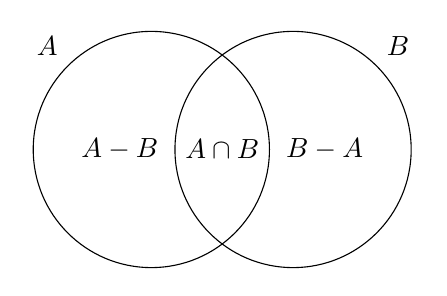
\begin{tikzpicture}
            \node [
                draw,
                circle,
                minimum size =3cm,
                label={135:$A$}
            ] (A) at (0,0){};
            \node [
                draw,
                circle,
                minimum size =3cm,
                label={45:$B$}
            ] (B) at (1.8,0){};
            \node at (0.9,0) {$A\cap B$};
            \node at (-0.4,0) {$A - B$};
            \node at (2.2,0) {$B - A$};
        \end{tikzpicture}\end{center}
        %% Answers
        \begin{enumerate}
            \item $A \cup B = \{
                1, 2, 3, 4, 5, 6, 8, 13
            \}$
            \item $A \cap B = \{
                2,8
            \}$
            \item $A - B = \{
                1, 3, 5, 13
            \}$
            \item $B - A = \{
                4, 6
            \}$
            \item $(A \cup B) - (A \cap B) = \{
                1, 3, 4, 5, 6, 13
            \}$
        \end{enumerate}
    \end{solution}
    %%%%%%%%%%%%%%%%%%%%%%%%%%%%%%%%%%%%%%%%%%%%%%%%%%%%%%%%%%%%%%%%
    % Question #6
    %%%%%%%%%%%%%%%%%%%%%%%%%%%%%%%%%%%%%%%%%%%%%%%%%%%%%%%%%%%%%%%%
    \item[6.]
    List all the elements of $\mathcal{P}(\mathcal{P}(\mathcal{P}(\emptyset))) - \mathcal{P}(\mathcal{P}(\emptyset)) + \mathcal{P}(\emptyset) - \emptyset$
    %%%%%%%%%%%%%%%%%%%%%%%%%%%% Solution %%%%%%%%%%%%%%%%%%%%%%%%%%%%
    \begin{solution}
        By definition, the power set of $S$ is the set of all subsets of the set $S$. Thus, the only element of a power set of an empty set will be an empty set itself.
        $$\mathcal{P}(\emptyset) = \{\emptyset\}$$
        Now, we do have an element that is an empty set which means we do not have an empty set for $\mathcal{P}(\emptyset)$. Using the definition of power set again, we can derive the followings.
        $$\mathcal{P}(\mathcal{P}(\emptyset)) = \{\{\emptyset\},\emptyset\}$$
        $$\mathcal{P}(\mathcal{P}(\mathcal{P}(\emptyset))) = \{
            \{\{\emptyset\},\emptyset\},
            \{\{\emptyset\}\},
            \{\emptyset\},
            \emptyset
        \}$$
        $$\textbf{Answer: }\mathcal{P}(\mathcal{P}(\mathcal{P}(\emptyset))) - \mathcal{P}(\mathcal{P}(\emptyset)) + \mathcal{P}(\emptyset) - \emptyset = \{
            \{\{\emptyset\},\emptyset\},
            \{\{\emptyset\}\},
            \emptyset
        \}$$
    \end{solution}


    
\end{enumerate}